% Part: sets-functions-relations
% Chapter: relations
% Section: trees

\documentclass[../../../include/open-logic-section]{subfiles}

\begin{document}

\olfileid[fa-IR]{sfr}{rel}{tre}
\olsection{درخت‌ها}

نوع خاصی از ترتیب جزئی که در همهٔ بخش‌های منطق نقشی مهم ایفا می‌کند
\emph{درخت} است. درخت‌های متناهی در بخش‌های مقدماتی منطق پدیدار می‌شوند:
برای نمونه، !!{formula}s را می‌توان بر حسب تجزیه‌شان به یک درخت نحوی
فهمید، و !!{derivation}s در بسیاری از دستگاه‌های !!{derivation} نیز
صورت درخت‌های متناهی دارند.
%
درخت‌های نامتناهی از همان اثبات قضیه‌های تمامیت برای منطق گزاره‌ای و
منطق مرتبهٔ اول پدیدار می‌شوند و در سراسر منطق ریاضی به کار می‌روند.

مفهوم مجموعه‌شناختی درخت پیوند نزدیکی با مفهوم درخت در نظریهٔ گراف
دارد. در زیر تصویری از یک درخت (متناهی) آمده است:

\begin{center}
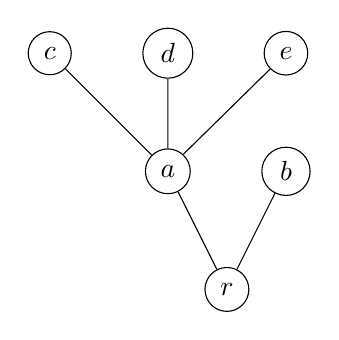
\begin{tikzpicture}[nodes={draw, circle}, -]
\node{$r$} [grow'=up]
    child { node {$a$} 
        child { node {$c$} }
        child { node {$d$} }
        child { node {$e$} }
    }
    child { node {$b$} };
\end{tikzpicture}
\end{center}

پایین‌ترین گره، یعنی~$r$، ریشه است. هر گره به‌جز $r$ دقیقاً یک گرهٔ
والد بلافاصله زیر خود دارد. رابطه‌ای را که گره~$x$ با گره~$y$ دارد،
هرگاه بتوان به $y$ با دنبال‌کردن یال‌ها رو به بالا از~$x$ رسید، می‌توان
چنین در نظر گرفت که $x$ یک \emph{نیای}~$y$ است.

رابطهٔ نیا در یک درخت، یک ترتیب جزئیِ اکید است. این نکته انگیزهٔ تعریف
مجموعه‌شناختی را فراهم می‌کند. برای بیان آن به دو مفهوم نیاز داریم.
یک \emph{کوچک‌ترین عضو} در مجموعهٔ~$A$ که با~$\le$ به‌طور جزئی مرتب
شده، !!a{element} $x \in A$ است چنان‌که برای هر $y \in A$ داشته باشیم
که~$x \le y$. یک مجموعه \emph{خوش‌ترتیب} به‌وسیلهٔ~$\le$ است اگر هر
زیرمجموعهٔ ناتهی آن کوچک‌ترین عضو داشته باشد.

\begin{defn}[درخت]
یک \emph{درخت} زوج $T = \tuple{A, \le}$ است، به‌طوری‌که $A$ مجموعه‌ای
است و $\le$ ترتیبی جزئی روی~$A$ است که یک کوچک‌ترین عضو یکتا
$r \in A$ دارد (که \emph{ریشه} نامیده می‌شود)، و برای هر $x \in A$،
مجموعهٔ $\Setabs{y}{y \le x}$ به‌وسیلهٔ~$\le$ خوش‌ترتیب است.
\end{defn}

\begin{defn}[جانشین‌ها]
فرض کنید $T = \tuple{A, \le}$ یک درخت باشد.
اگر $x,y \in A$، $x < y$، و هیچ $z \in A$ای وجود نداشته باشد که
$x < z < y$، آنگاه می‌گوییم $y$ یک \emph{جانشینِ}~$x$ است.
\end{defn}

جانشین‌های $x \in A$، \emph{فرزندان} آن نیز نامیده می‌شوند. اگر
$y$ جانشین~$x$ باشد، آنگاه $x$ را \emph{پیشین} یا \emph{والدِ}~$y$
می‌نامیم.

\begin{prop}
اگر $\tuple{A,\le}$ یک درخت باشد، آنگاه هر $x \in A$ به‌جز ریشه،
حداکثر یک پیشین دارد.
\end{prop}

\begin{proof}
  فرض کنید $y_1 < x$ و $y_2 < x$ و $y_1 \neq y_2$. آنگاه $\{y_1,
  y_2\} \subseteq \Setabs{z}{z<x}$. چون $\Setabs{z}{z<x}$
  به‌وسیلهٔ~$\le$ خوش‌ترتیب است، زیرمجموعهٔ $\{y_1, y_2\}$ از آن یک
  کوچک‌ترین عضو دارد که آشکارا باید یا $y_1$ یا~$y_2$ باشد. پس یا
  $y_1 \le y_2$ یا $y_2 \le y_1$. فرض کردیم $y_1 \neq y_2$؛ بنابراین
  در واقع یا $y_1 < y_2$ یا $y_2 < y_1$. چون فرض کردیم $y_1 < x$ و
  $y_2 < x$، افزون بر این یا $y_1 < y_2
  < x$ یا $y_2 < y_1 < x$. پس $y_1$ و $y_2$ نمی‌توانند هر دو
  پیشین‌های~$x$ باشند.
\end{proof}

\begin{defn}
گفته می‌شود درخت $T = \tuple{A, \le}$ \emph{نامتناهی} است اگر $A$ یک
مجموعهٔ نامتناهی باشد، و در غیر این صورت \emph{متناهی} است. اگر $T$
چنان باشد که هر $x \in A$ فقط شمار متناهی‌ای از جانشین‌ها داشته باشد، آنگاه
می‌گوییم $T$ \emph{با انشعاب متناهی} است.
\end{defn}

\begin{defn}[شاخه‌ها]
با داشتن درخت $T = \tuple{A, \le}$، یک \emph{شاخه} از~$T$ زنجیری
بیشینه در~$T$ است؛ یعنی مجموعه‌ای $B \subseteq A$ چنان‌که برای هر
$x, y \in B$، یا $x \le y$ یا $y \le x$، و برای هر
$z \in X \setminus B$، یک $u \in B$ وجود دارد چنان‌که نه
$z \le u$ و نه $u \le z$.
%
از $[T]$ برای نمایش مجموعهٔ همهٔ شاخه‌های $T$ استفاده می‌کنیم.
\end{defn}

\begin{ex}
یک نمونهٔ کلاسیک از درختی با انشعاب متناهی، \emph{درخت دودویی
نامتناهیِ} دنباله‌های متناهی از $0$ و~$1$ است که گاهی
$\{0,1\}^*$ یا~$\Bin^*$ نوشته می‌شود و با رابطهٔ امتداد $\sqsubseteq$
مرتب شده است (برای نمونه، $101 \sqsubseteq 101101$).
از آنجا که هر رشتهٔ دودویی را همواره می‌توان با افزودن
یک $0$ یا یک $1$ به انتهای آن امتداد داد، این درخت بی‌نهایت
عضو دارد: هر عضو~$s$ دقیقاً دو جانشین، یعنی $s0$ و~$s1$، دارد. ریشهٔ آن
دنبالهٔ تهی $\emptyseq$ است.
\end{ex}

\begin{ex}
کمی کلی‌تر، مجموعهٔ دنباله‌های متناهی از اعداد طبیعی~$\Nat^*$ با
رابطهٔ امتداد~$\sqsubseteq$ نیز یک درخت است. آشکارا با انشعاب متناهی
نیست: هر $s \in \Nat^*$ بی‌نهایت جانشین~$sn$ دارد، یکی برای هر
$n \in \Nat$. هر $A
\subseteq \Nat^*$ که نسبت به~$\sqsubseteq$ بسته باشد، یک
\emph{زیردرختِ}~$\Nat^*$ است. (یعنی $A$ چنان است که اگر $s \in A$
و $s' \sqsubseteq s$، آنگاه $s' \in A$ نیز.) همهٔ درخت‌های متناهی را
می‌توان به‌صورت زیردرخت‌های متناهیِ~$\Nat^*$ بازنمایی کرد.
\end{ex}

\begin{prop}[لم \foreignlanguage{english}{K\H{o}nig}]
اگر $T = \tuple{A,\le}$ درختی نامتناهی با انشعاب متناهی باشد،
آنگاه $T$ یک شاخهٔ نامتناهی دارد.
\end{prop}

حالت خاصی از لم \foreignlanguage{english}{K\H{o}nig} که به‌طور گسترده در نظریهٔ محاسبه‌پذیری به
کار می‌رود و \emph{لم ضعیف \foreignlanguage{english}{K\H{o}nig}} نام دارد، چنین است: هر زیردرخت
نامتناهی از $\{0,1\}^*$ یک شاخهٔ نامتناهی دارد.

\end{document}
